\section{Modell Anpassungen}
Das trainierte Modell der Walker Demo beherrscht jedoch nur die Fortbewegung in Blickrichtung. Durch diese Einschränkung lässt sich von der Steuerung mit WASD nur die W Komponente nutzen. Eine weitere große Einschränkung ist, das der Läufer nicht darauf trainiert ist stehen zu bleiben. Das resultiert darin das der Läufer fällt sobald der Nutzer keinen Tastaturinput gibt. Dieses Kapitel beschäftigt sich mit den Einschränkungen der Walker-Demonstration im Bezug auf unterschiedliche Bewegungsrichtungen.

\subsection{Versuch 4}
Im ersten Schritt wird getestet wie der Walker angepasst werden kann um die fehlenden Bewegungsabläufe in separaten Modellen zu erlernen.
Für das stehenbleiben wird die Zielgeschwindigkeit auf 0 gesetzt während das Ziel auf der Startposition befindet. Die Belohnungsfunktion der Demo hat dabei das Problem das durch die Zielgeschwindigkeit geteilt wird.\\
\begin{figure}[H]
  \centering  
  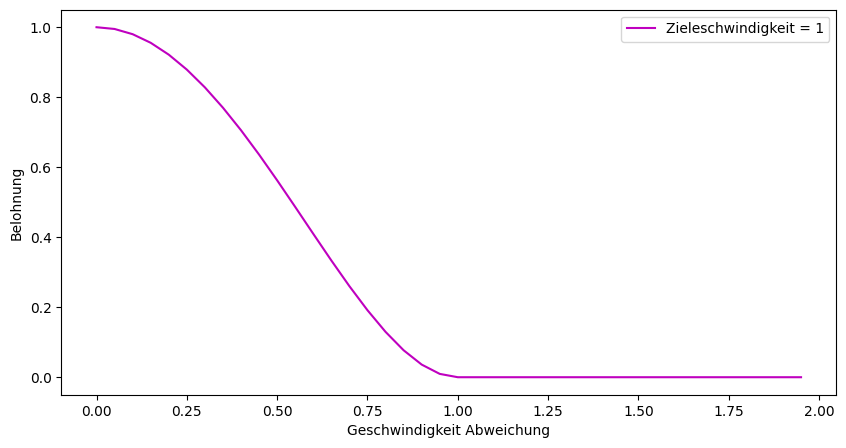
\includegraphics[scale=0.5]{img/match_velocity_original_vel1.png}
  \caption{Walker Demo Match Velocity Belohnungsfunktion}
  \label{fig:match_velocity_original_vel1}
\end{figure}
Die Abbildung \ref{fig:match_velocity_original_vel1} zeigt die Original Belohnungsfunktion ($R_V=(1 - (V_\delta / |\vec{Zielgeschwindigkeit}|)^2)^2$) für die Zielgeschwindigkeit von 1. \\
Um das zu vermeiden wurde das trainieren mit einer anderen Belohnungsfunktion getestet.
\begin{figure}[H]
  \centering  
  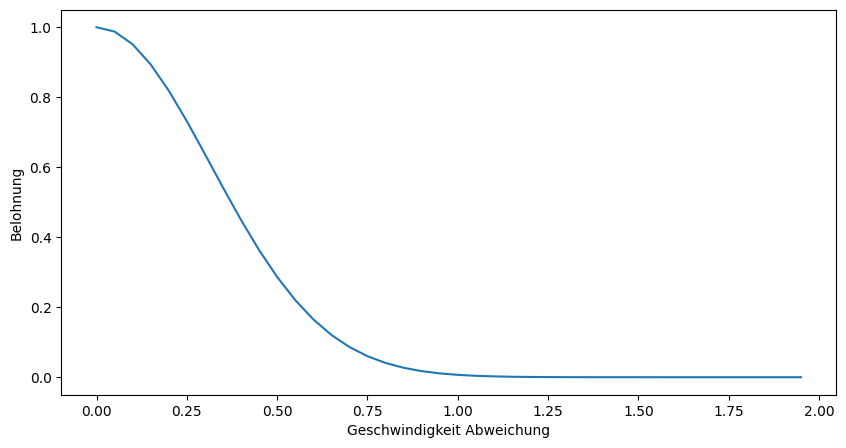
\includegraphics[scale=0.5]{img/match_velocity_exp.png}
  \caption{Neue Exponential Match Velocity Belohnungsfunktion}
  \label{fig:match_velocity_exp}
\end{figure}
Die Abbildung \ref{fig:match_velocity_exp} zeigt die neue Belohnungsfunktion ($R1_V=exp(5 \cdot (-V_\delta^2))$). Die neue Belohnungsfunktion ist inspiriert von den Belohnungsfunktionen des Papers "DeepMimic: Example-Guided Deep Reinforcement Learning of Physics-Based Character Skills".\cite{peng2018deepmimic}

Der Walker konnte mit der neuen Belohnungsfunktion lernen auf der Stelle zu stehen. Mit zufälliger Zielgeschwindigkeit zu einem Ziel zu laufen wie im Ursprünglichen Verhalten konnte damit jedoch nicht zufriedenstellend erlernt werden.

\begin{figure}[H]
  \centering  
  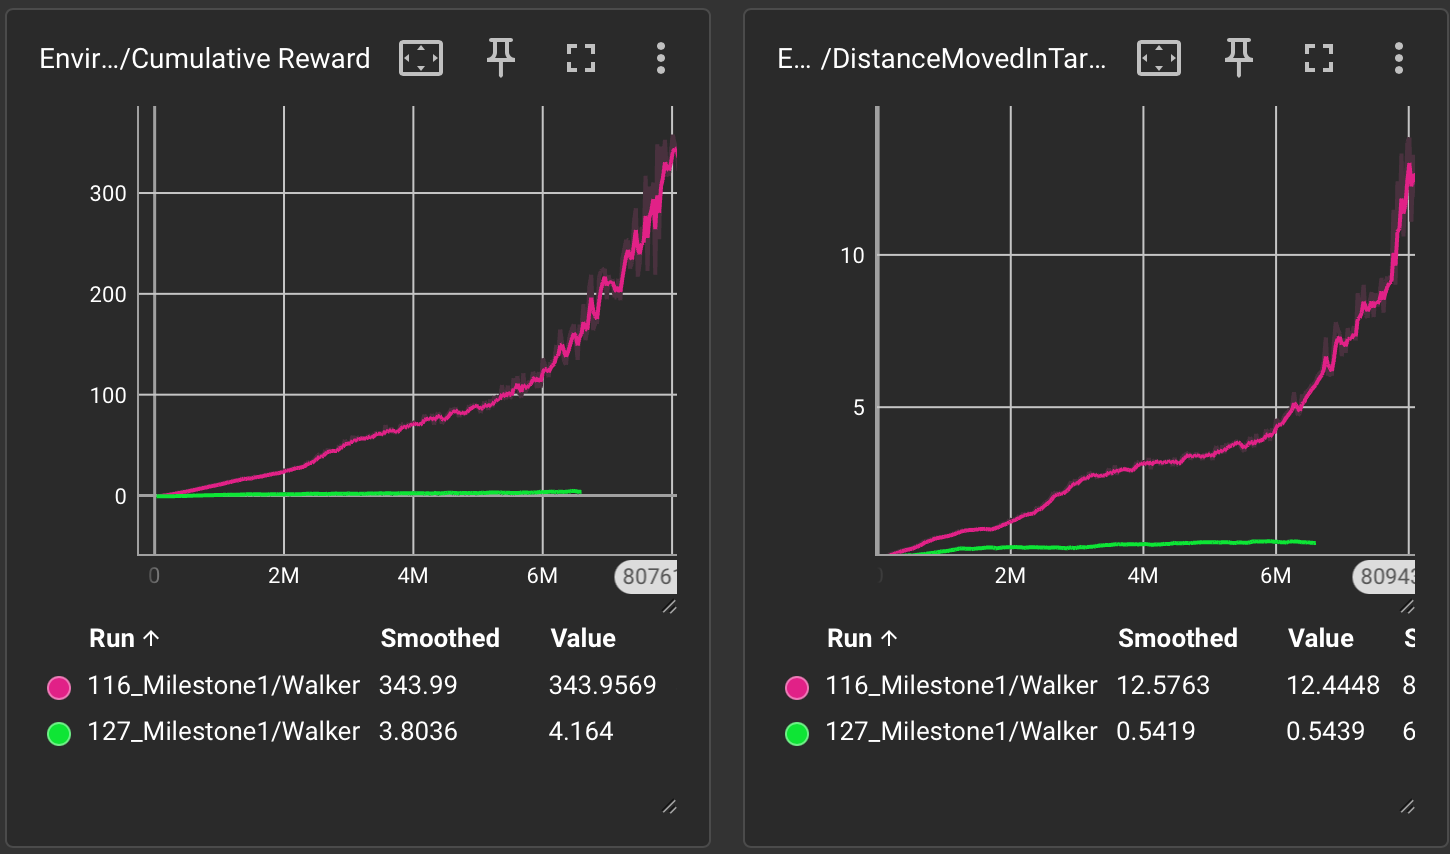
\includegraphics[scale=0.5]{img/training_exp_belohnung.png}
  \caption{Vergleich vorwärts laufen Exp Belohnung gegen Walker Demo Belohnung}
  \label{fig:training_exp_belohnung}
\end{figure}

Die Abbildung \ref{fig:training_exp_belohnung} zeigt mit der grünen Linie die Leistung der neuen Belohnungsfunktion und mit der pinken Linie die Leistung der Walker Demo Belohnungsfunktion. Nachfolgender Vergleich der Belohnungsfunktionen zeigt das die Ursprüngliche Belohnungsfunktion durch das Teilen mit der Zielgeschwindigkeit die Sensitivität der Funktion je nach Zielgeschwindigkeit beeinflusst. Daraus folgt das bei steigender Zielgeschwindigkeit eine größere Abweichung der Geschwindigkeit geduldet wird. Diese Anpassung verbessert die Generalisierung zwischen den wechselnden Geschwindigkeiten um ein vielfaches.

\begin{figure}[H]
  \centering  
  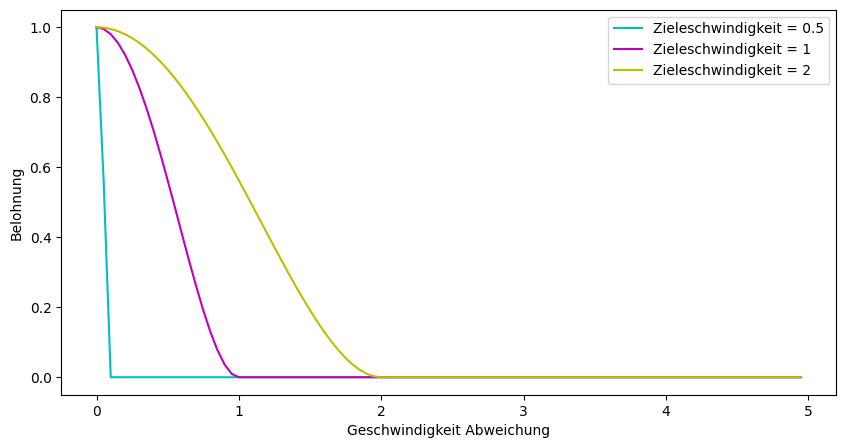
\includegraphics[scale=0.5]{img/match_velocity_original_vergleich.png}
  \caption{Vergleich der Walker Demo Belohnungsfunktion unter verschiedenen Zielgeschwindigkeiten}
  \label{fig:match_velocity_original_vergleich}
\end{figure}

Mit dieser Erkenntnis wurde eine neue Anpassung untersucht. In der folgenden Anpassung blieb die Belohnungsfunktion weitestgehend Unverändert. Lediglich das obere Limit ab welchem die Funktion eine Belohnung von 0 annimmt, wurde auf ein minimum von 0.1 beschränkt. Somit konnte sicher gestellt werden das im Bereich der normalen Fortbewegung keine Veränderung auftritt. Bei allen Zielgeschwindigkeiten unter 0.1 wurde somit 0.1 als maximale Abweichung genutzt.\\
$V_\delta=Clip(|\vec{Geschwindigkeit} - \vec{Zielgeschwindigkeit}|, 0, |\vec{Zielgeschwindigkeit}|)$ \\
$V_\delta=Clip(|\vec{Geschwindigkeit} - \vec{Zielgeschwindigkeit}|, 0, max(0.1, |\vec{Zielgeschwindigkeit}|))$ \\



stehen bleiben:
wenn Distance < slowDownDistance dann je nach Distanz die Geschwindigkeit verringern -> agent bleibt vor ziel stehen bzw. kreist um ziel

extra Laufrichtungen:
-getrennte Modelle und Modell live wechseln problem mit seitwärts laufen und vermutlich schlechter Übergang bei Wechsel
-ein Modell mit Laufrichtung als one hot encoding in Beobachtung mit Lektion für verschiedene Laufrichtung -> kann nicht von vorwärtslaufen auf andere Richtung generalisieren bzw. anpassen (vergisst vorheriges verhalten) schränkt Bewegung auf feste Bewegungsrichtungen ein (vorwärts, rechts, links, rückwärts)
-extra Ziel für Blickrichtung:
  -Ziel zufällig gesetzt mit Winkel Begrenzung von agent zu ziel -> Winkel ändert sich bei Bewegung
  -Blickziel setzen bei Episodenwechsel oder Ziel erreicht -> ändert sich zu häufig das Agent verhalten nicht lernt
  -Blickziel und Laufziel nur neu setzen wenn Durchschnittliche Blickbelohnung > Grenzwert -> zu schwer bzw. dauert zu lange, Agent veralten schon zu sehr vertieft um es groß zu ändern
  -Walker lernt auf Boden zu schauen da Blickrichtung nach unten näher an Blickrichtung Ziel ist wenn sich das Ziel hinter dem Walker befindet
  -Extra Belohnung für aufrechte Blickrichtung
  -Blickziel wird jedes Physikupdate neu gesetzt um Winkel gleich zu behalten
  -Blickziel neu setzen wenn bestimmte Zeit auf Ziel geschaut (mit Spherecast) -> funktioniert nicht schlecht aber bei längerem training hört der Agent auf das Blickziel zu erreichen